\subsection{Variability aware Performance Prediction}\label{sec:VAPP}

The following section is based upon \citet{VariabilityAwarePerformancePredictionJianmeiSigmundApel}.\\
Variability aware Performance Prediction (\VAPP) is a statistics based approach to performance prediction. With the help of random sampling and \CART s a simple yet effective predictor can be build. In their own tests \citet{VariabilityAwarePerformancePredictionJianmeiSigmundApel} reached an average precision of 94\% whilst using a sample as large as the ones \AFID would be using under the PW heuristic. Further tests conducted by \citet{FasterDiscoveryofFasterSystemConfigurationsSiegmund2017} with the same sample size showed an accuracy of 92.4\%. 


\begin{wrapfigure}{r}{.5\linewidth}
	\vspace{-1\baselineskip}
	\setlength\belowcaptionskip{-\baselineskip}
	\includegraphics[page=3,clip,trim=11cm 13.5cm 1.5cm 10.25cm, width=\linewidth ]{Paper/VariabilityAwarePerformancePredictionAStatisticalLearningApproach}
	\caption{Overview of the Approach of Variability aware Performance Prediction \cite{VariabilityAwarePerformancePredictionJianmeiSigmundApel}}.
	\label{fig:VAPPOverview}
\end{wrapfigure}

\subsubsection[Basic Idea]{\textnormal{The} basic idea} of variability aware performance prediction can be seen in \autoref{fig:VAPPOverview}.

Two cycles can be found. 

The first cycle is outside of the dashed box and describes the basic input-output behaviour of a predictor. A user configures a new configuration $\x$ for System $A$ and asks the predictor (dashed box) for a prediction. It replies with a quantitative prediction for $\x$'s performance.

In the second cycle a actual prediction is generated based on decision rules which themselves are inturn created by simplifying a performance model (a \CART). Random sampling is used to learn the performance model.
\\\\
Like other approaches, the target of variability aware performance prediction is to get accurate predictions with only using a small sample for the creation of the performance model.

\FloatBarrier %forces the float to appear below the subsubsection
\subsubsection{Statistical Methods}\label{sec:VAPPMethods} are used to perform the actual computation. First of all a configuration is defined as an $N$-tuple $(x_1,x_2,x_3,...,x_N)$, where $N$ is the number of all available features. Each $x_i$ represents a feature and can either have the value 1 or 0 depending on whether the feature is selected or not. An actual configuration example would be $\x_j = (x_1=1,x_2=0,x_3=1,\dots,x_N = 1)$. All valid configurations of a system are denoted as $\X$.\\

\VAPP~uses the tupel definition of a configuration. It further defines that for each configuration of $\mathcal{C}$ an actual performance value $y_j$ can be assigned. $\Y$ denotes the performance of all configurations of a system.\\
For formal correctness it is assumed that each option of a configuration actually influences the performance of the system. Otherwise a \CART could not be applied.

Combining $\Y_\X$ with $\X_\mathcal{C}\subset\mathcal{C}$ gives a sample $S$. $\Y_\X$ are the to $\X_C$ associated and measured performance values. Now the two problems arise that \VAPP tries to solve:
\begin{enumerate}
	\item Predict the performance of the not measured configurations $\hat{=}\;\X\backslash\X_\mathcal{C}$.
	\item Find a function $f$ that shows the correlation between $\X_\mathcal{C}$ and $Y_\X$ and that makes each predicted performance $f(\x)$ of $\x$ as close as possible to its actual performance.\\	
	\begin{equation}
	f : \mathcal{C} \rightarrow  \mathbb{R} \text{ such that} \sum_{\x,y \in S} L(y,f(\x)) \text{ is minimal}
	\end{equation}\\
	 $L$ is a loss function to penalize errors in prediction.
\end{enumerate}
This is done with the help of CART. All sample configurations get categorized into a binary trees leafs. A configurations selection of features determines its location in the tree. The distribution of samples inside the tree is determined with the goal of minimizing the total prediction errors per segment (sub-trees). An example tree can be found in \cref{fig:VAPPExampleTree}.
For each leaf one can determine the \textit{local model} $\ell$
\begin{equation}
	\ell_{S_i} = \frac{1}{|S_i|} \sum_{y_j \in S_i} y_j
\end{equation}
As a loss function to penalize the prediction errors \citet{VariabilityAwarePerformancePredictionJianmeiSigmundApel} choose the sum of squared error loss:
\begin{equation}
	\sum_{y_j \in S_i} L(y_i,\ell_{S_i}) = \sum_{y_j \in S_i} (y_j - \ell_{S_i})^2
\end{equation}
Therefore the best split for a segment $S_i$ is found when
\begin{equation*}
\sum_{y_j \in S_{iL}} L(y_i,\ell_{S_{iL}}) + \sum_{y_j \in S_{iR}} L(y_i,\ell_{S_{iR}})
\end{equation*}
is minimal. To prevent \textit{under}- or \textit{overfitting}\cite{ElementsOfStatisticalLearning} the recursive splitting has to be stopped at the right time. This is possible by manual parameter tuning or using a empirical-determined automatic terminator. \\
Now to the actual calculation of the quantitative prediction. Assuming there are $q$ leafs in our tree than $f(\mathrm{x})$ is defined as:
\begin{equation}\textsl{}
f(\mathrm{x})=\sum_{i=1}^{q} \ell_{S_i}I(\mathrm{x}\in S_i)
\end{equation}
where $I(\mathrm{x}\in S_i)$ is an indicator function to indicates that $\mathrm{x}$ belongs to a leaf $S_i$.\\
For the example of \autoref{fig:VAPPExampleTree} $f(\mathrm{x})$ unwraps to:
\begin{align*}
f(x) = 255&* I(x_{14}=1,x_7=0)\\[-0.1cm]
	 + 268&* I(x_{14}=1,x_7=1)\\[-0.1cm]
	 + 402&* I(x_{14}=0,x_{15}=1,x_3=0)\\[-0.1cm]
	 + 508&* I(x_{14}=0,x_{15}=1,x_3=1)\\[-0.1cm]
	 + 571&* I(x_{14}=0,x_{15}=0,x_3=1)\\[-0.1cm]
	 + 626&* I(x_{14}=0,x_{15}=0,x_3=0)
\end{align*}
Every possible configuration $\mathrm{x}$ is associated with a leaf of the tree. Therefore $f(\mathrm{x})$ can always be applied.\\
For their Experiment \citet{VariabilityAwarePerformancePredictionJianmeiSigmundApel} test the same software systems as \citet{AutomatedFeatureDetectionSiegmund2012} (\cref{sec:AFID}). They also compare their prediction results with the results produced by SPLConquerer under \AFID.\\
Unlike \AFID~the size of a sample for variability aware performance prediction can be chosen freely. \citet{VariabilityAwarePerformancePredictionJianmeiSigmundApel} use 4 different sample sizes based on the size of the program. For a program with $N$ features they use samples the size of $N,2N,3N \text{ and } M$. $M$ is the amount of configurations measured by SPLConquerer's using the \hyperref[lab:PW]{PW heuristic}.
It is found that the prediction accuracy increases linear with the size of the sample. It is also found that for using a small sample with the size of $N$ the prediction accuracy was at 92\%. However for Berkeley DB (C) the prediction rate with $N$ sized samples was at 112.4$\pm$354.6\%\footnote{$\pm$354.6 indicates the standard deviation}. This results into an average accuracy of only 28.6$\pm$68.9\%. Using a sample size of $M$ significantly improves the average prediction accuracy to 93.8\%.\\
Further \citet{VariabilityAwarePerformancePredictionJianmeiSigmundApel} comparer their approach with \AFID. This can be done since $N$ also equals the amount of configurations measured by the \hyperref[lab:FW]{FW heuristic}.\\
As already established variability aware performance prediction is not accurate for small sample sizes so it is no surprise that \AFID~with the \hyperref[lab:FW]{FW heuristic} performace better at $20.3\pm21.2$\% with a sample size of $N$. However, when using samples of size $M$ SPLConquerer's \hyperref[lab:PW]{PW heuristic} only reaches an average precision of 90.9\% compared to the already mentioned 93.9\% of \citet{VariabilityAwarePerformancePredictionJianmeiSigmundApel}'s approach.
Using the \hyperref[lab:HO]{HO} or \hyperref[lab:HS]{HS heuristic} of \AFID can produce a precision of up to 95\% but requires more measurements. This is not covered by \cite{VariabilityAwarePerformancePredictionJianmeiSigmundApel}.
%TODO vllt selbst prüfen?
